\subsection{Kempe-chains}

In the five color theorem we worked with a vertex that had 5 neighbors. We used chains of 2 colors between its neighbors to \textit{flip} the colors of these neighbors, creating a new coloring. If we return to the problem of finding a common ring coloring for a ring configuration $\confg$ on $R$ and the graph $M+R$, we do not know much of the ring colorings in $\Phi(M+R)$. All we know, are the guaranteed colorings from contracting the ring $R$. To obtain more guaranteed colorings, we can use the same trick of flipping the colors of vertices on the same chain. Therefore, let us define \textit{Kempe-chains}.

\begin{definition}
    Let $G_{ab}(x)$ be the subgraph consisting of all the vertices colored $ab$ in the coloring $x$ of $G$.
    Then the \emph{Kempe-chain} $\kappa_{ab}(v)$ or \emph{$ab$-chain} of the vertex $v$ is the component of $G_{ab}(x)$ that contains $v$. 
\end{definition}

\begin{figure}[!ht]
    \centering
    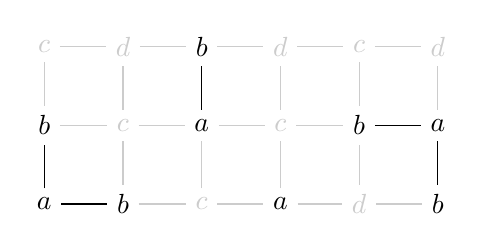
\begin{tikzpicture}[scale=1]
        \node (x11) at (0, 0) { $a$ };
        \node (x12) at (1, 0) { $b$ };
        \node[opacity=0.2] (x13) at (2, 0) { $c$ };
        \node (x21) at (0, 1) { $b$ };
        \node[opacity=0.2] (x22) at (1, 1) { $c$ };
        \node (x23) at (2, 1) { $a$ };
        \node[opacity=0.2] (x31) at (0, 2) { $c$ };
        \node[opacity=0.2] (x32) at (1, 2) { $d$ };
        \node (x33) at (2, 2) { $b$ };
        \node (y11) at (3, 0) { $a$ };
        \node[opacity=0.2] (y12) at (4, 0) { $d$ };
        \node (y13) at (5, 0) { $b$ };
        \node[opacity=0.2] (y21) at (3, 1) { $c$ };
        \node (y22) at (4, 1) { $b$ };
        \node (y23) at (5, 1) { $a$ };
        \node[opacity=0.2] (y31) at (3, 2) { $d$ };
        \node[opacity=0.2] (y32) at (4, 2) { $c$ };
        \node[opacity=0.2] (y33) at (5, 2) { $d$ };

        \draw (x11) -- (x12);
        \draw[opacity=0.2] (x12) -- (x13);

        \draw[opacity=0.2] (x21) -- (x22);
        \draw[opacity=0.2] (x22) -- (x23);
        \draw[opacity=0.2] (x31) -- (x32);
        \draw[opacity=0.2] (x32) -- (x33);

        \draw (x11) -- (x21);
        \draw[opacity=0.2] (x21) -- (x31);
        \draw[opacity=0.2] (x12) -- (x22) -- (x32);
        \draw[opacity=0.2] (x13) -- (x23);
        \draw (x23) -- (x33);

        \draw[opacity=0.2] (y11) -- (y12) -- (y13);
        \draw[opacity=0.2] (y21) -- (y22);
        \draw (y22) -- (y23);
        \draw[opacity=0.2] (y31) -- (y32) -- (y33);

        \draw[opacity=0.2] (y11) -- (y21) -- (y31);
        \draw[opacity=0.2] (y12) -- (y22) -- (y32);
        \draw (y13) -- (y23);
        \draw[opacity=0.2] (y23) -- (y33);

        \draw[opacity=0.2] (x13) -- (y11);
        \draw[opacity=0.2] (x23) -- (y21);
        \draw[opacity=0.2] (x33) -- (y31);
    \end{tikzpicture}
    \caption{The components of $G_{ab}(x)$ for a planar graph $G$ and its coloring $x$ are highlighted. We write $\chain{u}{v}{ab}$ or $u \in \kappa_{ab}(v)$ if $u$ and $v$ are on the same component.}
    \label{fig:kempetut}
\end{figure}

We can flip the colors of a chain $\kappa_{ab}(v)$ without breaking the current coloring. Imagine in your head how you can swap the chains in Figure \ref{fig:kempetut} for example. This is the trick to creating new guaranteed ring colorings in $\Phi(M+R)$.

Now, suppose that we are guaranteed that the coloring $abab$ is in $\Phi(M+R)$. If we want to flip any Kempe-chains on $abab$, then it is necessary to have information on them. This information is not obvious from the coloring $abab$ itself. To add this information, we  may consider two cases, one in which a chain is present, and another in which it is not. To visualise the Kempe-chains that are present on a coloring like $abab$, we may draw lines between vertices like

\begin{equation}
    \scheme{a,b,a,b}{13d}, \quad\quad \scheme{a,b,a,b}{24c}, \quad\quad \scheme{a,b,a,b}{13c-}.
\end{equation}

From this notation, it is visible at glance what the structure is of the ring coloring $abab$. A ring coloring together with knowledge of Kempe-chains we call a \textit{scheme}. In the left-most scheme for example, we see $\chain{v_1}{v_3}{ad}$. In the middle scheme, we see $\chain{v_2}{v_4}{bc}$ and in the right-most scheme, we see that $v_1$ and $v_3$ are not connected by an $ac$-chain.

\begin{definition}
    Given a coloring $x$ of a planar graph $G$ and the colors on its ring $x(R)$. The \emph{scheme} on $R$ of $x$ consists of $x(R)$ with knowledge whether $u \in \kappa_{ab}(v)$ for two ring vertices $u,v \in R$ and colors $ab$.
\end{definition}

\begin{figure}[!h]
    \centering
    \begin{tikzpicture}[scale=1.0, mid arrow/.style={
        postaction={ decorate, decoration={ markings, mark=at position 0.6 with { \arrow[black]{>>} } } } }]

        \node[circle, fill, scale=0.015cm, opacity=0.2] (v) at (0, 0) { };
        \node[circle, fill, scale=0.015cm, label=above:$a$] (l1) at (0, 1) { };
        \node[circle, fill, scale=0.015cm, label=right:$b$] (l2) at (0.9, 0.30) { };
        \node[circle, fill, scale=0.015cm, label=below:$c$] (l3) at (0.6, -0.77) {};
        \node[circle, fill, scale=0.015cm, label=below:$a$] (l4) at (-0.6, -0.77) {};
        \node[circle, fill, scale=0.015cm, label=left:$b$] (l5) at (-0.9, 0.30) {};
        \node[circle, fill, scale=0.015cm, label=above:$c$] (c1) at (0.7, 1) {};
        \node[circle, fill, scale=0.015cm, label=right:$a$] (c2) at (1.32, 0.68) {};
        \node[circle, fill, scale=0.015cm, label=right:$c$] (c3) at (1.45, 0.05) {};
        \node[circle, fill, scale=0.015cm, label=right:$a$] (c4) at (1.1, -0.49) {};
        \draw[mid arrow] (l1) -- (l2);
        \draw (l2) -- (l3) -- (l4) -- (l5) -- (l1);
        \draw (l1) -- (c1) -- (c2) -- (c3) -- (c4) -- (l3);
        \draw[opacity=0.2] (l1) -- (v);
        \draw[opacity=0.2] (l2) -- (v);
        \draw[opacity=0.2] (l3) -- (v);
        \draw[opacity=0.2] (l4) -- (v); 
        \draw[opacity=0.2] (l5) -- (v);
        \node (impl) at (3, 0) { $\hspace{1cm} \implies \hspace{0.3cm} \begin{matrix}
            \scheme{a,b,c,a,b}{ 13a } \\
            \scheme{a,b,c,a,b}{ 25d- }
        \end{matrix}$ };
        
    \end{tikzpicture}
    \caption{Two ring schemes that are derived from a graph coloring. }
    \label{fig:schemes}
\end{figure}

We will often make a case dinstinction on the Kempe-chains in the scheme of a ring coloring. We consider a case in which the scheme has the chain, and a case in which it has not. We rarely ever know \textit{all} the Kempe-chains of a scheme, but this is also never necessary. Given the information of just one Kempe-chain in a scheme, we can start \textit{reconfiguring} the colors of the ring by flipping Kempe-chains. This results in a new scheme with different ring colors. We say that one scheme \textit{implies} another scheme.

\begin{definition}
    Given two schemes $x$ and $y$. We say that $x \compat y$ if $x=y$ or $y$ can be obtained from $x$ by flipping a Kempe-chain.
\end{definition}

\begin{equation*}
    \begin{aligned}
    \circled{1}\quad\quad \scheme{a,b,c,a,b}{ 13a } &\compat \scheme{a,b,c,a,\textbf{d}}{{13a}}, \\
    \circled{2}\quad\quad \scheme{a,b,c,a,b}{ 25d- } &\compat \scheme{a,d,c,a,\textbf{d}}{{25d-}},\\
    \circled{3}\quad\quad \scheme{a,b,c,a,b}{ 13a } &\compat \scheme{\textbf{c},b,\textbf{a},\textbf{c},b}{{13a}}.
    \end{aligned}
\end{equation*}

For the two schemes from Figure \ref{fig:schemes}, we have given two implied schemes above (change is highlighted). To deduce these implied colorings, we followed a few simple rules.

\begin{enumerate}
    \item The two vertices colored $b$ are seperated by the $ac$-chain $\kappa_{ac}(v_1)$. Therefore, the $bd$-chain $\kappa_{bd}(v_5)$ can not possibly connect with $v_2$. This results in only $v_5$ being recolored to $d$ if we flip this chain.
    \item It is now directly given that $\kappa_{bd}(v_5)$ does not connect to $v_1$, therefore we may flip $v_5$ to $d$ in the same way as in the first case.
    \item Now we know $v_1$ and $v_3$ are in the same $ac$-chain. Because $v_4$ neighbors $v_3$ on the ring, it will also be included in this chain. Since all three are on $\kappa_{ac}(v_1)$, flipping this chain results in all their colors to be flipped.
\end{enumerate}

Refer to these examples whenever a step of implying colorings in a proof is confusing. It will be a key concept for the remainder of the paper.